\documentclass[aps,letterpaper,11pt]{revtex4}

\usepackage{graphicx}
\usepackage{float}
\usepackage{verbatim}
\usepackage{amsmath}
\usepackage{amssymb}

\newcommand{\labno}{9}
\newcommand{\labtitle}{Developing a New Amusement Park Ride for Joy Ride^{TM}}
\newcommand{\authorname}{Kevin Truong}
\newcommand{\professor}{Dr. Melanie Lutz}
\newcommand{\classno}{Physics 006}
\newcommand{\labpartners}{Sean Casey, Kevin Castillo, and Dulce Payan}
\newcommand{\submitdate}{April 25,2017}

\begin{document}

\begin{titlepage}
\begin{center}
\hspace{-136mm}\boxed{{\Large \textsc{Lab No. \labno}}}\\\vspace{30mm}
{\Large \textsc{\labtitle} \\ \vspace{4pt}}
\rule[13pt]{\textwidth}{1pt}\\ \vspace{150pt}
{\large By: \authorname \\ \vspace{10pt}}
Lab Partners: \labpartners \\
Instructor: \professor \vspace{10pt} \\
Solano Community College\\ \classno \\ \vspace{10pt}
\submitdate
\end{center}
\end{titlepage}

\section{Abstract}

In this experiment the $\mu_k$ of the ramp was found by analyzing 3 trials where we applied an initial force causing the cart to move, and the friction of the ramp slowed the cart down to a stop. The average $\mu_k$ was 0.0120. When the ramp was inclined, the angle between the ramp and the table was $8.12^o$ Then the theoretical acceleration as the cart moved up the ramp was calculated which was 0.530$\frac{m}{s^2}$ and the theoretical acceleration as the cart was moving down the ramp was calculated which was 0.317$\frac{m}{s^2}$; these calculations were found using the derived equations that were made prior to the experiment. When the experiment was actually ran, the experimental acceleration as the cart moved up the ramp was 0.512$\frac{m}{s^2}$ and the experimental acceleration as the cart moved down the ramp was 0.341$\frac{m}{s^2}$. Then the percent error between the experimental values and the theoretical values were calculated. the percent error of the acceleration as the cart was moving up the ramp was 3.43\% and the percent error of the acceleration as the cart moved down the ramp was 7.57\%.


\section{Introduction}

Up to this point we have only analyzed movement and forces on "frictionless" surfaces, but in real life friction is all around us. Causing bodies to slow down and stop, friction acts opposite to the direction of motion of the object. There is two types of friction: static friction and kinetic friction. Static friction is when a body is at rest, the force needed to overcome static friction is greater than the force needed to overcome kinetic friction. The formula for static friction is represented by: $f_s \leq \mu_sN$ and the formula for kinetic friction is represented by: $f_k = \mu_kN$. In this experiment we will be analyzing kinetic friction and the kinetic coefficient of kinetic friction. Conservation of energy is an important concepts when analyzing work done by friction. The energy in a system must be conserved, so when we know friction will be in the system the work done by friction must be considered when analyzing the conservation of enery equation. It's important to note that the acceleration that was indicated throughout the experiment would be negative when describing the acceleration of the cart and positive when describing the acceleration of the hanging mass, this is due to how the axis is placed on the free body diagrams of the cart and hanging mass.

\section{Experimental Details}

Equipments for this experiment includes a ramp, cart, 0.05kg mass, string, pulley, motion detector, and computer. The ramp was the medium for the cart to move on, the surface of the ramp had friction. The cart was pushed up and down the ramp, it is the object being analyzed throughout this experiment. The 0.05kg mass was attached to the cart using a string and was hung from a pulley, it accelerates with the cart. The String kept the cart and the hanging mass linked together. The pulley was used to keep a smooth movement between the cart and the hanging mass. The motion detector was used to calculate the acceleration, velocity, and position of the moving cart. The computer was used to process the collected data of the motion detector through the Logger Pro program. 

For part A of the experiment, we found the kinetic coefficient of friction of the track by simply pushing the cart on the ramp when it was straight horizontal with the table. We did this by using the motion detector analyzing, on the computer, how the cart slowed down due to the friction of the ramp. The following is the diagram for part A, where the cart was pushed and analyzed using the motion detector; we did this three times and found the average coefficient of friction to have a more accurate calculation of the coefficient of friction.

\begin{center}
\underline{Diagram 1}\\

\textit{Diagram 1: Setup for the part A of the experiment}\\
\end{center}

For part B of the experiment, the ramp was set up as an incline by using a rod stand; so the ramp had some angle $\theta$. The cart was attached to a hanging mass by using a string and the string was hung from a pulley. The cart was givin an initial push up the incline and the cart slowed down going up the incline and eventually began coming down the incline. This part of the experiment analyzed the tension and acceleration of the cart as it moved up and as it moved down the incline, all of the motion of the cart was collected using the motion detector. The following diagram is the setup for part B of the experiment:

\newpage

\begin{center}
\underline{Diagram 2}\\

\textit{Diagram 2: Setup for part B of the experiment}\\
\end{center}

\section{Results and Analysis}

\subsection{Effective Coefficient of Kinetic Friction}

For part A of the experiment, the kinetic coefficient of friction($\mu_k$) was found. The cart was pushed with an initial force and the friction of the ramp slowed the cart down to a stop. This motion was recorded by the motion detector and the data was organized by Logger Pro. The equation to solve for the coefficient of friction was derived prior to the experiment was:

$$ \mu_k = \frac{v_0^2}{2gd}$$
\begin{center}
NOTE: Complete derivation in the appendix.
\end{center}

The cart was pushed three separate times and the kinetic coefficient was calculated for each trial, and the average value for the kinetic coefficient of friction was calculated and used for a more accurate value. 

\subsubsection{First Push}

For the first push, figure 1 shows the distance vs. time graph of the motion of the cart. 

\newpage

\begin{center}

\textit{Figure 1: The distance vs. time graph for the first push for $\mu_k$}\\
\end{center}

Analyzing this graph using the tools of Logger Pro, the initial position of the cart was 0.743m away from the motion detector and when the cart slowed down and stopped due to friction the final position was 1.497m. The total distance that the cart traveled for this first push was 0.754m.

Figure 2 shows the velocity as it slows down due to friction:

\newpage

\begin{center}

\textit{Figure 2: The Velocity Vs. Time graph for the first push, showing it as it slows down due to friction.}\\
\end{center}

Figure 2 was analyzed using the tools in the Logger Pro Program and the initial velocity when it begins slowing down due to friction was 0.413$\frac{m}{s}$. From figure 1 and figure 2 the following information on the cart can be concluded:

\begin{center}
\underline{First Push Data Table}\\
\begin{tabular}{|c|c|}
\hline
$x_0$ & 0.743m \\
\hline
$x_f$ & 1.497m \\
\hline
d & 0.754m\\
\hline
$v_0$ & 0.413$\frac{m}{s}$\\
\hline
\end{tabular}
\end{center}

Plugging all of the information found into the equation derived:

$$ \mu_k=\frac{(0.413\frac{m}{s})^2}{2(9.8\frac{m}{s^2})(0.754m)} = 0.0115$$

\subsubsection{Second Push}

For the second push, figure 3 shows the distance vs. time graph of the motion of the cart. 

\begin{center}
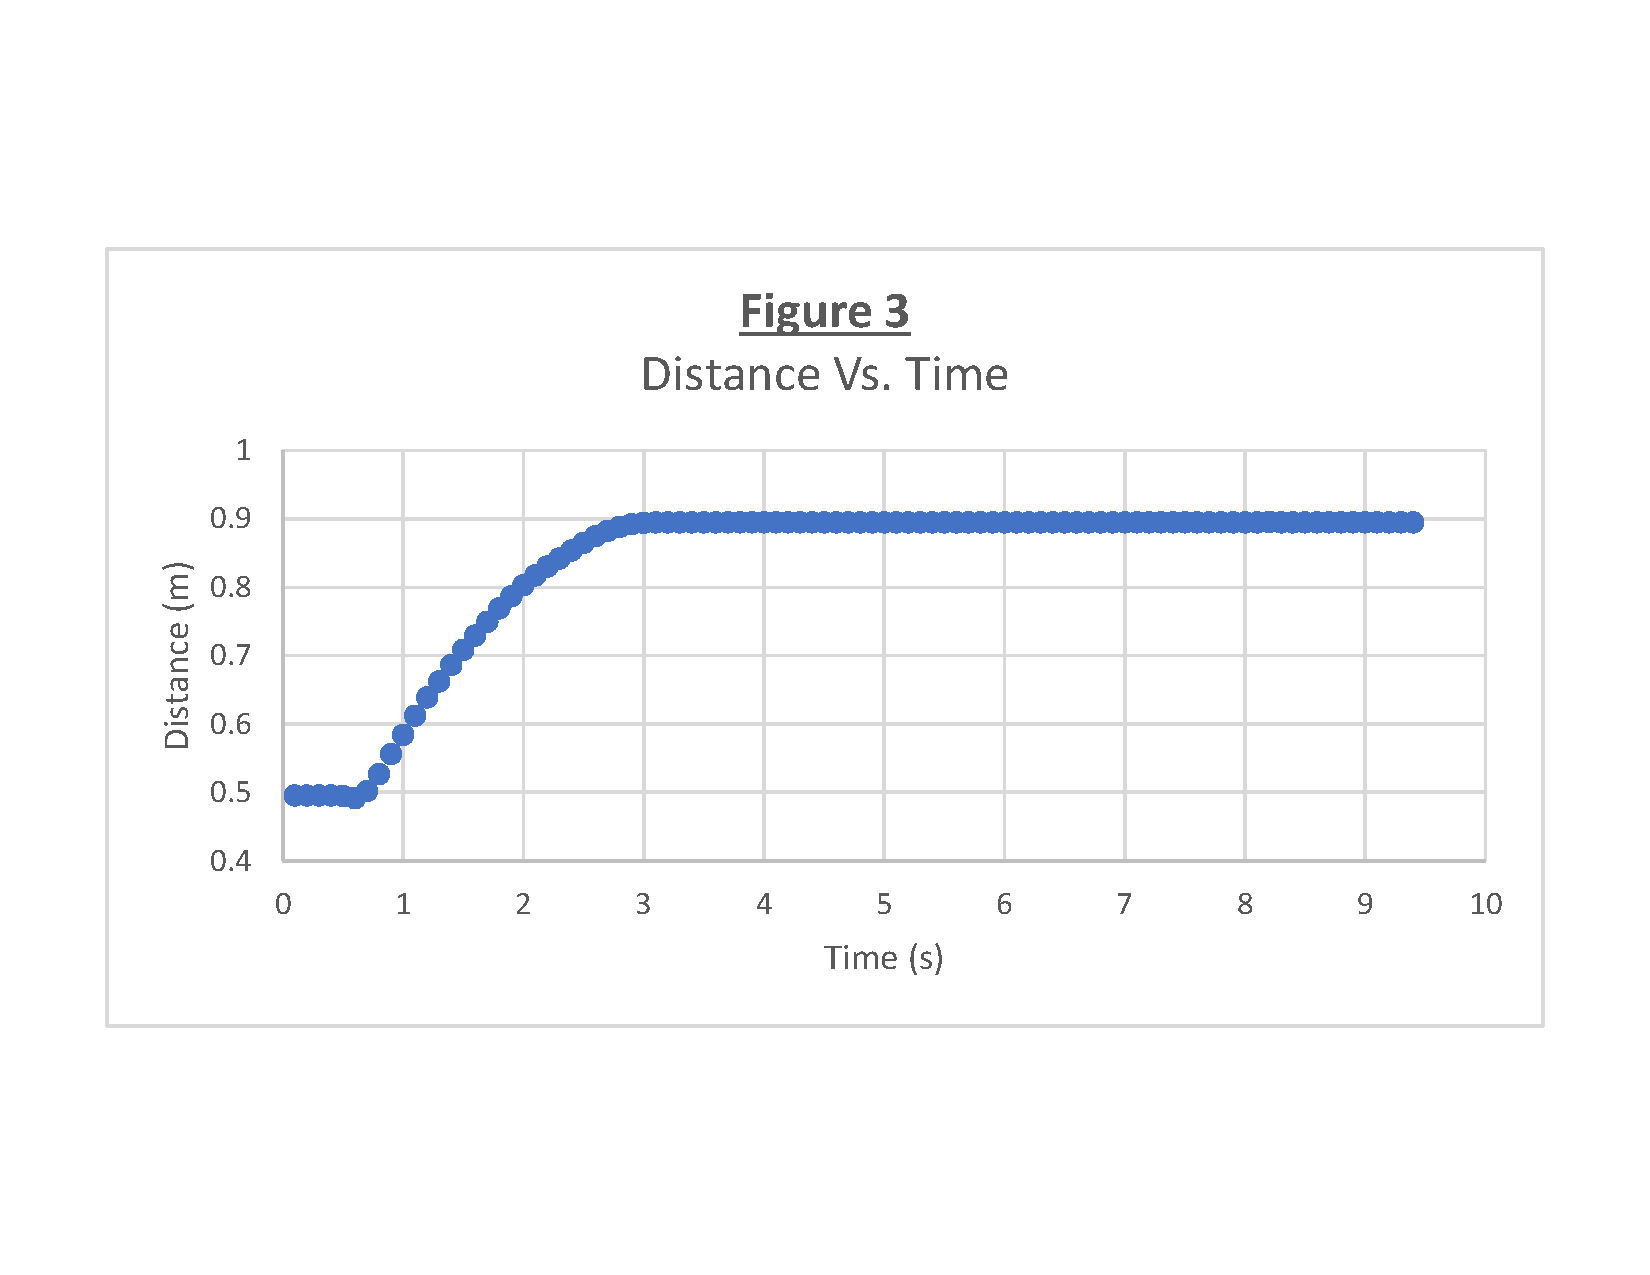
\includegraphics[width=5in]{DistanceVsTimeGraphForMuSecond.pdf}\\
\textit{Figure 3: The distance vs. time graph for the second push for $\mu_k$}\\
\end{center}

Analyzing this graph using the tools of Logger Pro, the initial position of the cart was 0.584m away from the motion detector and when the cart slowed down and stopped due to friction the final position was 0.895m. The total distance that the cart traveled for this first push was 0.311m.

Figure 4 shows the velocity as it slows down due to friction:

\begin{center}

\textit{Figure 4: The Velocity Vs. Time graph for the second push, showing it as it slows down due to friction.}\\
\end{center}

Figure 4 was analyzed using the tools in the Logger Pro Program and the initial velocity when it begins slowing down due to friction was 0.277$\frac{m}{s}$. From figure 3 and figure 4 the following information on the cart can be concluded:

\begin{center}
\underline{First Push Data Table}\\
\begin{tabular}{|c|c|}
\hline
$x_0$ & 0.584m \\
\hline
$x_f$ & 0.895m \\
\hline
d & 0.311m\\
\hline
$v_0$ & 0.277$\frac{m}{s}$\\
\hline
\end{tabular}
\end{center}

Plugging all of the information found into the equation derived:

$$ \mu_k=\frac{(0.277\frac{m}{s})^2}{2(9.8\frac{m}{s^2})(0.311m)} = 0.0126$$

\subsubsection{Third Push}

For the third push, figure 5 shows the distance vs. time graph of the motion of the cart. 

\begin{center}

\textit{Figure 5: The distance vs. time graph for the third push for $\mu_k$}\\
\end{center}

Analyzing this graph using the tools of Logger Pro, the initial position of the cart was 0.560m away from the motion detector and when the cart slowed down and stopped due to friction the final position was 1.186m. The total distance that the cart traveled for this first push was 0.626m.

Figure 6 shows the velocity as it slows down due to friction:

\begin{center}

\textit{Figure 6: The Velocity Vs. Time graph for the third push, showing it as it slows down due to friction.}\\
\end{center}

Figure 6 was analyzed using the tools in the Logger Pro Program and the initial velocity when it begins slowing down due to friction was 0.382$\frac{m}{s}$. From figure 5 and figure 6 the following information on the cart can be concluded:

\begin{center}
\underline{First Push Data Table}\\
\begin{tabular}{|c|c|}
\hline
$x_0$ & 0.560m \\
\hline
$x_f$ & 1.186m \\
\hline
d & 0.626m\\
\hline
$v_0$ & 0.382$\frac{m}{s}$\\
\hline
\end{tabular}
\end{center}

Plugging all of the information found into the equation derived:

$$ \mu_k=\frac{(0.382\frac{m}{s})^2}{2(9.8\frac{m}{s^2})(0.626m)} = 0.0119$$

\subsubsection{Average of all three pushes}

The average kinetic coefficient of friction was then calculated using the three values calculated for the three different pushed:

\begin{center}
Average value of $\mu_k = \frac{0.0115 + 0.0126 + 0.0119}{3} = \boxed{0.0120}$
\end{center}

\subsection{Inclined Atwood's Machine}

Now that the kinetic coefficient of friction was found for the ramp, we can now use it when analyzing the tension of the string or the acceleration of the cart and hanging mass. 

When the ramp was inclined up the $\theta$ between the ramp and the table top was $8.12^o$.

initially the cart is given a push up the incline, when analyzing the motions and forces on the cart($m_1$) and hanging mass($m_2$), it's necessary to consider the free body diagram of both.

\begin{center}

\end{center}

While the cart is moving the incline because of the initial force applied, the direction of acceleration is down the incline because it's slowing down as it is moving up the incline.

As the stops, when moving up the incline, because the acceleration is causing it to slow down, the cart begins moving down the incline. When analyzing the forces on the cart and hanging mass as they move down the incline, it's necessary the free body diagram of both.

\begin{center}

\end{center}

As the cart is moving down the incline, the direction of acceleration is still down the ramp because it's increasing in speed as it travels down the ramp.

The acceleration going up the ramp is greater than the acceleration going down the ramp because when the cart is moving up the ramp friction is point in the direction of acceleration and when the cart is moving down the ramp, friction is point in the opposite direction of acceleration. Essentially friction is "helping" pull the cart down the ramp when the cart is moving up the ramp. 

If there was no friction, than the acceleration moving up the ramp would be the same as the acceleraion moving down the ramp because friction isn't "helping" or "fighting against" the movement of the cart. 

When derived the equation of the acceleration when the cart is moving up the ramp ($a_{up}$) is:

$$ a_{up}=\frac{m_1g(sin\theta+\mu_kcos\theta)-m_2g}{m_1+m_2}$$

\begin{center}
NOTE: The lengthy derivation is in the Appendix\\
\end{center}

Also the derived equation of the acceleration when the cart is moving down the ramp ($a_{down}$) is:

$$ a_{down}=\frac{m_1g(sin\theta-\mu_kcos\theta)-m_2g}{m_1+m_2}$$

\begin{center}
NOTE: The lengthy derivation is in the Appendix\\
\end{center}

when comparing the equation for $a_{up}$ and $a_{down}$ it is easy to see that $a_{up} > a_{down}$. Both equations are very similar except $a_{up}$ has $(sin\theta + \mu_kcos\theta)$ while $a_{down}$ has $(sin\theta - \mu_kcos\theta)$.

$$ (sin\theta + \mu_kcos\theta) \geq (sin\theta - \mu_kcos\theta)$$

The equations would only be equal if there was no friction (meaning $\mu_k = 0$), which agrees with the statement that was made earlier: that if there was no friction the accelerations up and down would be the same.

The mass of the cart was found using a scale, the mass of the cart was 0.532kg.

Now that we have all of the necessary information to calculate $a_{up}$ and $a_{down}$, it's possible to just plug the information into the derived equation and solve for the theoretical accelerations. 

When plugging in $m_1 = 0.532kg$, $\theta = 8.12^o$, $\mu_k = 0.012$, $g = 9.8\frac{m}{s^2}$, and $m_2 = 0.05kg$ into the equations for $a_{up}$ and $a_{down}$, the $\boxed{theoretical \hspace{1mm} a_{up} = 0.530\frac{m}{s^2}}$ and the $\boxed{theoretical  \hspace{1mm}a_{down} = 0.317\frac{m}{s^2}}$.

Running the actual experiment of giving the cart an initial push and allowing it to stop and roll back down the ramp gave us Figures 7, 8, and 9 that were distance vs. time graph, velocity vs. time graph, and acceleration vs. time graph of the cart's movement, respectively. 

\begin{center}

\textit{The distance vs. Time graph for the cart on the inclined ramp}\\

\textit{The Velocity vs. Time graph for the cart on the inclined ramp}\\

\textit{The Acceleration Vs. Time graph for the cart on the inclined ramp}\\
\end{center}


Using the tools in the Logger Pro Program the mean values of acceleration for the region of the graph of acceleration vs. time where it is approximately constant yielded an $a_{up} = 0.512\frac{m}{s^2}$ and $a_{down} = 0.341\frac{m}{s^2}$. 

Comparing the experimental values to the theoretical values the percent error could be calculated. The equation for percent error is:

$$ \% error = |\frac{a_{experimental} - a_{Theoretical}}{a_{theoretical}}|$$

When plugging in the values into the equation above, the $\% error$ of $a_{up}$: 3.43\%. The \% error of $a_{down}$: 7.57\%. The percent error indicates that there was some disparity between the experimental values and the theoretical values, but the percent error is not that drastic. 

\section{Discussion} 

The experiment showed that the acceleration as the cart moved up the ramp was greater than the acceleration as the cart moved down the ramp. The percent error of the experiment could have been caused by the motion detector and how it picks up the motion of the cart, a solution to this problem might be to increase the sample amount that the motion detector reads per second. It's important to note that the acceleration that was indicated throughout the experiment would be negative when describing the acceleration of the cart and positive when describing the acceleration of the hanging mass, this is due to how the axis is placed on the free body diagrams of the cart and hanging mass. 

\section{Appendix}

Derivation 1 (solving for $\mu_k$):

\begin{center}

\end{center}

Looking at the FBD of the cart on the flat ramp, we can do the summation of forces in the y-direction:

$$ \sum_{}^{}F_y = 0$$

It's equal to 0 because there is no movement in the y-direction.

$$ N - mg = 0$$

$$ N = mg$$

The equation for friction is:

$$ f = \mu_kN$$

from our summation of forces in the y-direction:

$$ f = \mu_k(mg)$$

By conservation of energy this statement must be true:

$$ W_f + KE_1 = KE_2$$

Where the first state of KE is after the initial push and the second state of KE is when the cart stops. Therefore $KE_2$ will be equal to 0 because the equation for $KE = \frac{1}{2}mv^2$ and when the cart is stopped $v = 0$. 

$$ W_f = -KE_1$$

where $W_f = fd$, friction over some distance d. It's important to note that work done by friction is always negative! 

$$ -fd = -\frac{1}{2}mv_0^2$$

$$ -(\mu_k(mg)d) = -\frac{1}{2}mv_0^2 $$

after isolating $\mu_k$:

$$ \mu_k = \frac{v_0^2}{2gd}$$

Derivation 2 (solving for $a_{up}$):

\begin{center}

\end{center}

The summation of forces in the x-direction of the cart is $T-f-m_1gsin\theta = -m_1a_{up}$ and the summation of forces in the y-direction of the cart is $N = m_1gcos\theta$.
The summation of forces in the y-direction on the hanging mass is $T-m_2g = m_2a_{up}$ or $T = m_2(a_{up} + g)$. Note: $f = \mu_kN$

Solving for T in the summation of forces in the y-direction for the hanging mass and plugging it in for the T in the summation of forces in the x-direction of the cart:

$$ m_2(a_{up}+g)-\mu_k(m_1gcos\theta)-m_1gsin\theta = -m_1a_{up}$$

Then through some simple arithmetic, it's possible to solve for $a_{up}$:

$$ a_{up} = \frac{m_1g(sin\theta+\mu_kcos\theta)-m_2g}{m_1+m_2}$$

Derivation 3 (solving for $a_{down}$):

\begin{center}

\end{center}

The summation of forces in the x-direction of the cart is $T+f-m_1gsin\theta = -m_1a_{down}$ and the summation of forces in the y-direction of the cart is $N = m_1gcos\theta$.
The summation of forces in the y-direction on the hanging mass is $T-m_2g = m_2a_{down}$ or $T = m_2(a_{down} + g)$. Note: $f = \mu_kN$

Solving for T in the summation of forces in the y-direction for the hanging mass and plugging it in for the T in the summation of forces in the x-direction of the cart:

$$ m_2(a_{down}+g)+\mu_k(m_1gcos\theta)-m_1gsin\theta = -m_1a_{down}$$

Then through some simple arithmetic, it's possible to solve for $a_{down}$:

$$ a_{down} = \frac{m_1g(sin\theta-\mu_kcos\theta)-m_2g}{m_1+m_2}$$





\section{References}

\hspace{-6.5mm}
Force and Acceleration III Physics 06 Lab, Dr. Melanie Lutz\\



\end{document}
